\chapter{Condizionamento dell'Ingresso}

%--------------------------------------------------------------------------------------------

\section{Convertitore Lineare-Esponenziale}

%--------------------------------------------------------------------------------------------

Vogliamo ora analizzare la sezione di circuto che soddisfa la specifica sulla modalità
$1V/Octave$ dell'ingresso, ovvero il circuito in grado di convertire una tensione
lineare in una esponenziale.

%--------------------------------------------------------------------------------------------

\subsection*{Analisi del Circuito}

%--------------------------------------------------------------------------------------------

Per l'applicazione si sfrutta la caratteristica esponenziale intrinseca del transistor
bipolare:

\begin{displaymath}
    i_e\approx i_c=I_se^{\left(\frac{v_{be}}{V_T}-1\right)}
    \approx I_se^{\left(\frac{v_{be}}{V_T}\right)}
\end{displaymath}

\begin{figure}[ht]
    \centering
    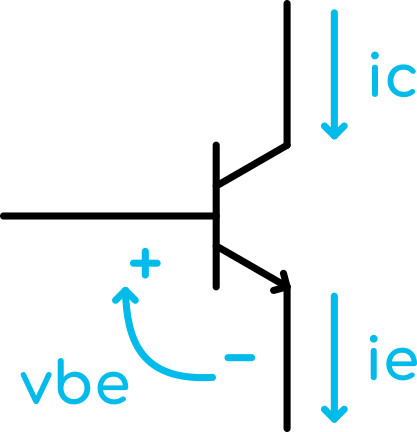
\includegraphics{circuits/single_transistor_circuit.png}
    \caption{BJT}
    \label{bjt}
\end{figure}

dove $V_T$ (o potenziale termico) e $I_s$ (o corrente di saturazione) sono variabili in
funzione della temperatura, ad ogni modo nella nostra analisi considereremo $V_T$ costante
a $26mV$.

Per rimuovere dall'equazione $I_s$ invece, si collegano 2 transistor (idealmente nello
stesso chip, in modo che siano il più possibile simili tra loro e termicamente accoppiati)
in configurazione a coppia differenziale:
\medskip

\begin{figure}[ht]
    \centering
    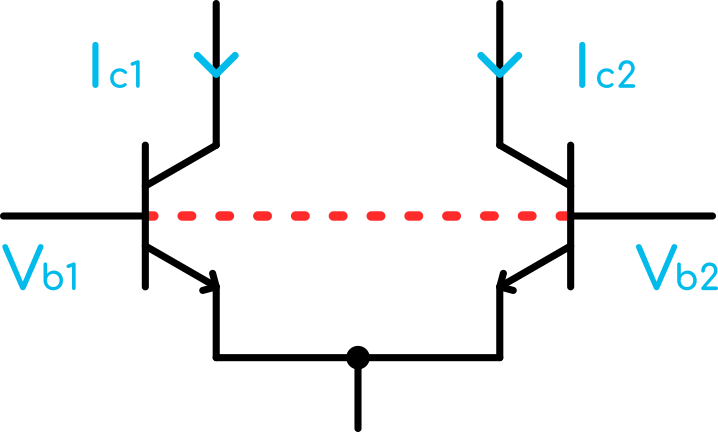
\includegraphics{circuits/differential_pair_circuit.png}
    \caption{Coppia differenziale a BJT}
    \label{differential_pair_circuit}
\end{figure}

per la quale vale la seguente relazione:

\begin{displaymath}
    \frac{i_{c2}}{i_{c1}}=\frac{I_s e^{\left(\frac{v_{be2}}{V_T}\right)}}{I_s e^{\left(\frac{v_{be1}}{V_T}\right)}}
    \qquad
    \rightarrow
    \qquad
    i_{c2}=i_{c1}e^{\left(\frac{v_{be2}-v_{be1}}{V_T}\right)}=i_{c1}e^{\left(\frac{v_{b2}-v_{b1}}{V_T}\right)}
\end{displaymath}

dove risulta evidente che la dipendenza da $I_s$ viene completamente rimossa.

A questo punto, apportiamo alcune modifiche al circuito:

\begin{figure}[ht]
    \centering
    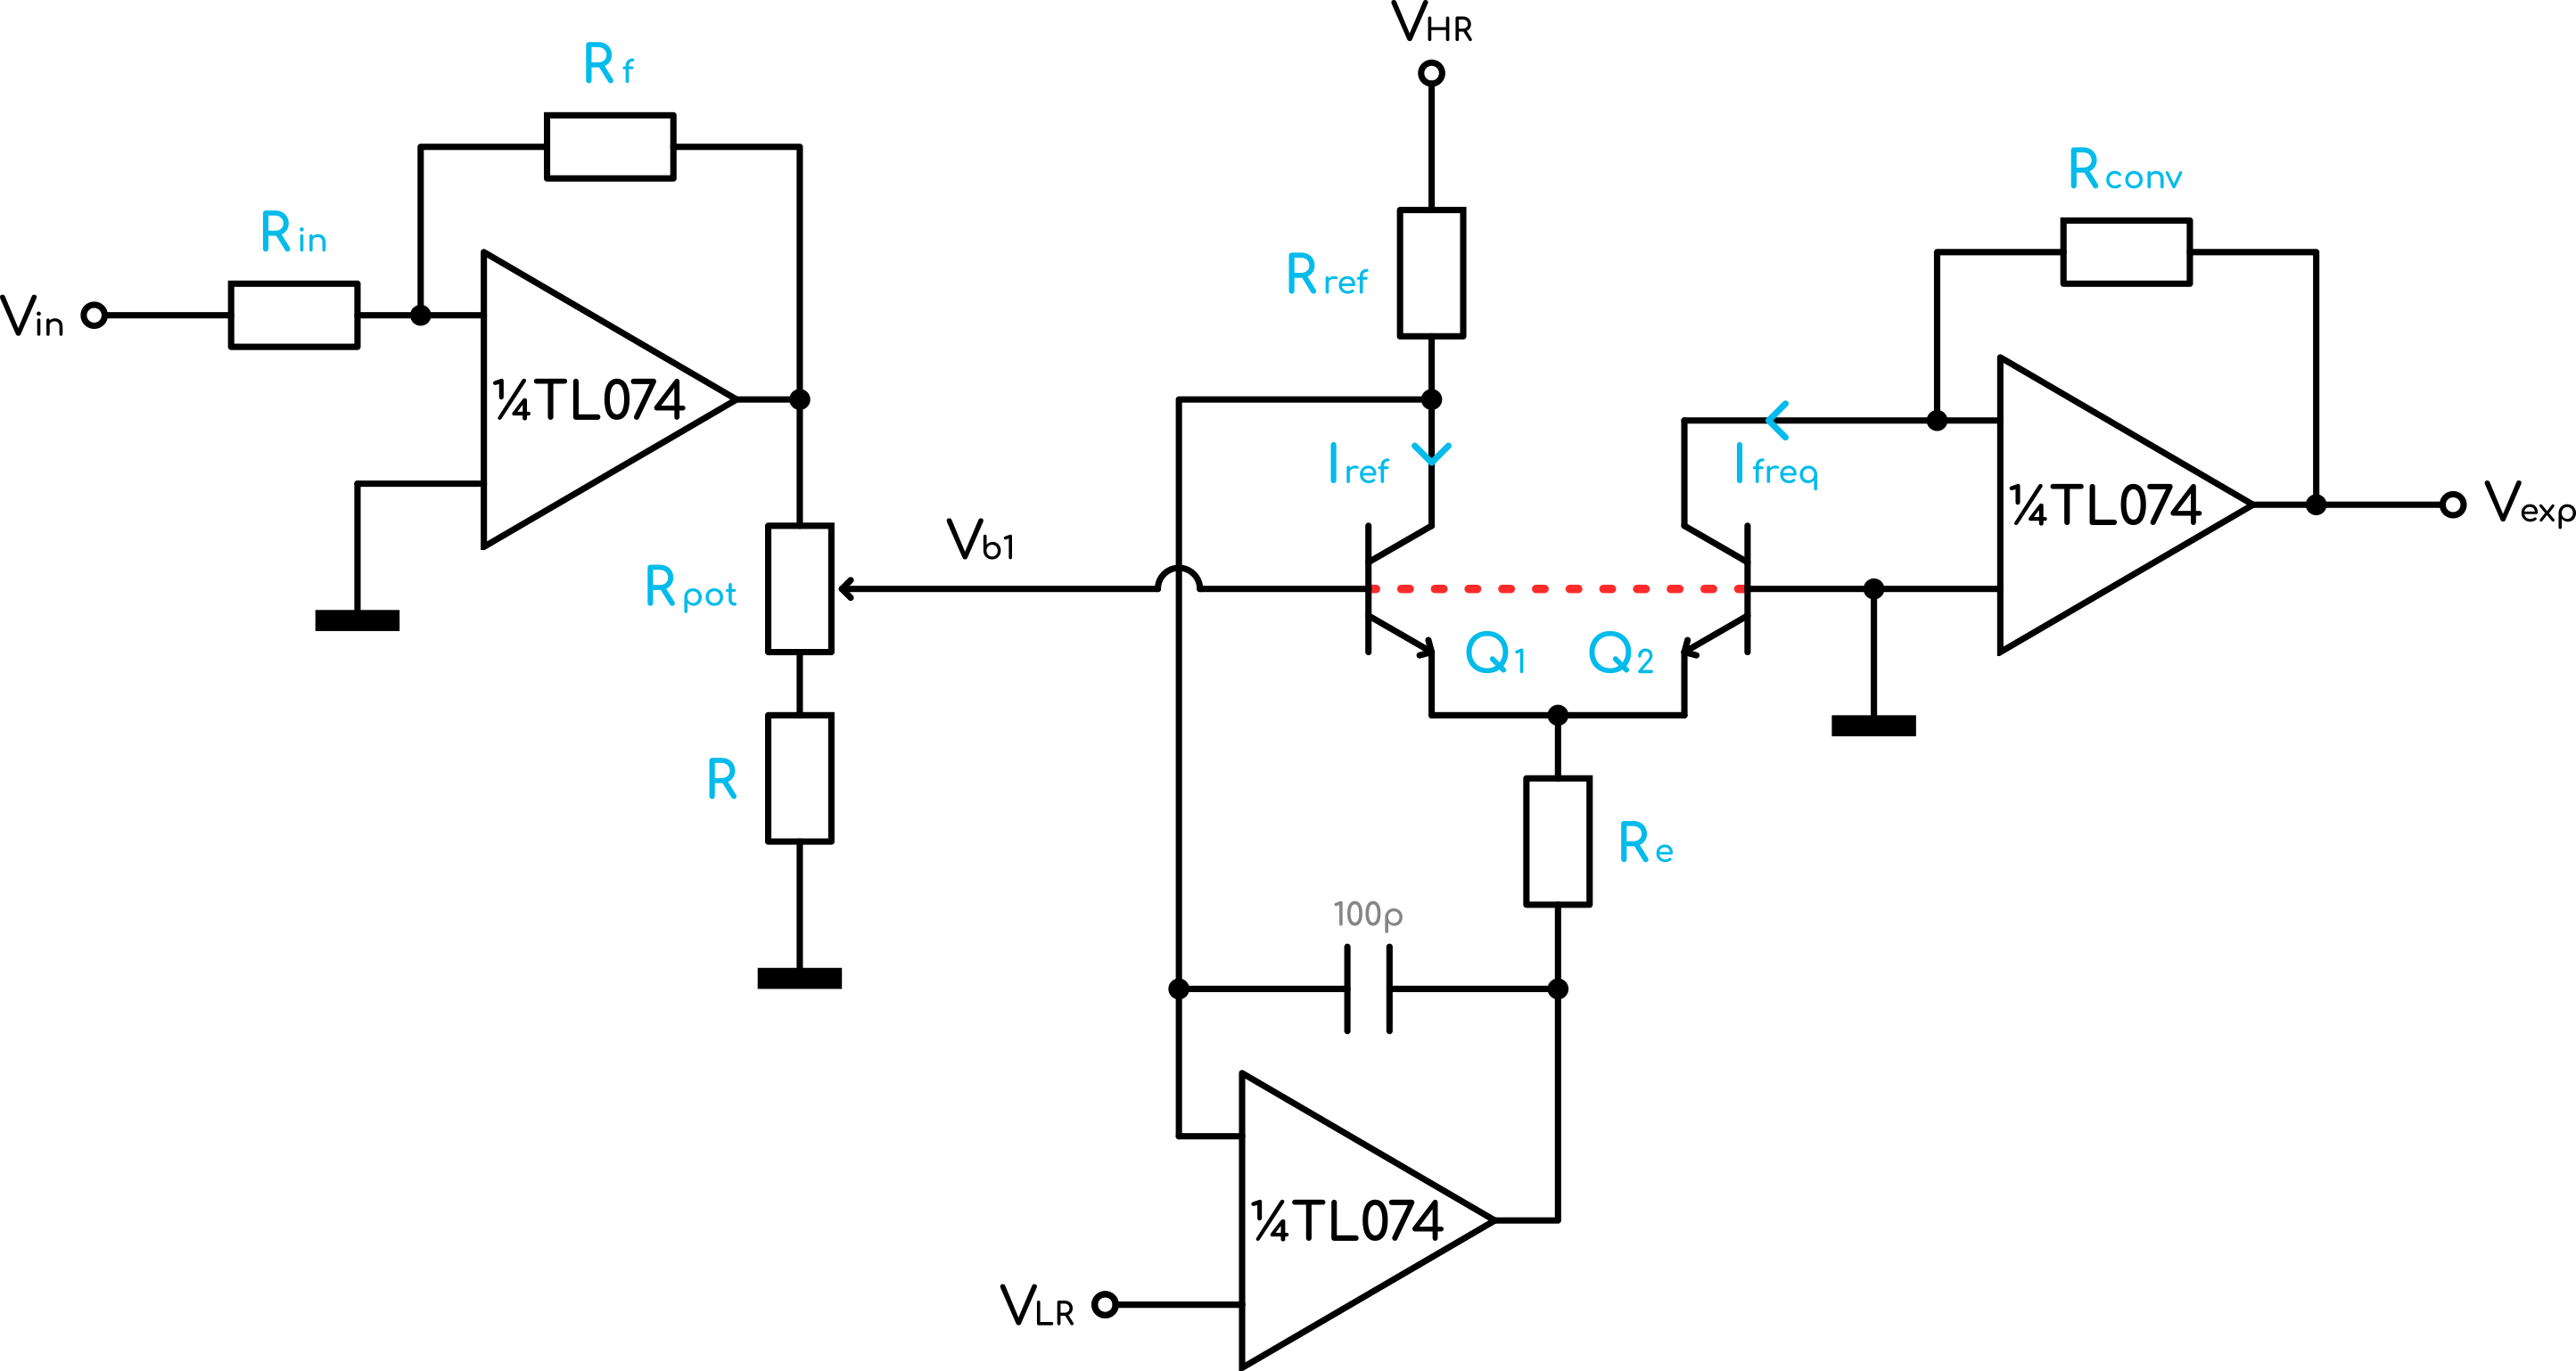
\includegraphics{circuits/exponential_converter_circuit.png}
    \caption{Convertitore tensione lineare - corrente esponenziale}
    \label{exponential_converter_circuit}
\end{figure}

dove l'operazionale di sinistra si occupa di invertire il segno della tensione di ingresso
per avere un valore positivo all'esponente, mentre quello di destra si occupa di mantenere
costante la corrente di riferimento $I_{ref}$.

Valgono quindi:

\begin{displaymath}
    i_{freq}=I_{ref}e^{-\frac{v_{b1}}{V_T}}
\end{displaymath}

\begin{displaymath}
    I_{ref}=\frac{V_{HR}-V_{LR}}{R_{ref}}
\end{displaymath}

Ora per completare il tutto basta aggiungere un convertitore corrente-tensione al collettore
di $Q_2$, legando cosi $V_{in}$ a $V_{out}$ con la seguente relazione:

\begin{displaymath}
    V_{out}=R_f\cdot i_{freq}=
    R_f\cdot I_{ref}e^{-\frac{v_{b1}}{V_T}}=
    R_f\cdot \frac{V_{HR}-V_{LR}}{R_{ref}}e^{-\frac{s\cdot V_{in}}{V_T}}
\end{displaymath}

% circuito completo con IVC figura 4

%--------------------------------------------------------------------------------------------

\subsection*{Dimensionamento e Scelta dei Componenti}

%--------------------------------------------------------------------------------------------

Passiamo quindi al dimensionamento dei componenti, in modo da imporre al circuito il
comportamento voluto.

Come prima cosa calcoliamo il valore del guadagno $s$ dell'amplificatore invertente.
Si vuole:

\begin{displaymath}
    i_{freq}=I_{ref}e^{-\frac{s\cdot V_{in}}{V_T}}
    \qquad
    \rightarrow
    \qquad
    2i_{freq}=I_{ref}e^{-\frac{s\cdot[V_{in}+\Delta V_{in}]}{V_T}}
\end{displaymath}

qundi un raddoppio della corrente $i_{freq}$ per ogni variazione $\Delta V_{in}=1V$.
Allora possiamo riscrivere le due relazioni nel seguente modo:

\begin{displaymath}
    2=e^{-\frac{s\cdot\Delta V_{in}}{V_T}}
    \qquad
    \rightarrow
    \qquad
    ln(2)=-\frac{s\cdot\Delta V_{in}}{V_T}
    \qquad
    \rightarrow
    \qquad
    -s=\frac{V_T\cdot ln(2)}{\Delta V_{in}}
\end{displaymath}

e sostituendo i valori otteniamo:

\begin{displaymath}
    -s=\frac{26mV\cdot 0.6931}{1V}\approx-0.018\approx-\frac{1}{55.5}
\end{displaymath}

valore che può essere diviso nel seguente modo:

\begin{displaymath}
    s=\bar{s}\cdot\hat{s}=\frac{2k\Omega}{100k\Omega}\cdot\frac{440\Omega}{490\Omega}
    \approx 0.018
\end{displaymath}

quindi:

% circuito amplificatore completo figura 5

\begin{itemize}
    \item $R_f = 2k\Omega$;
    \item $R_{in} = 100k\Omega$;
    \item $R_{pot} = 100\Omega$;
    \item $R = 390\Omega$;
\end{itemize}

impostiamo i valori di $V_{HR}=+12V$ e $V_{LR}=0V$.

%--------------------------------------------------------------------------------------------

\subsection*{Risultati Pratici e Misure}

%--------------------------------------------------------------------------------------------

testo

%--------------------------------------------------------------------------------------------

\section{Somma di più Ingressi}

%--------------------------------------------------------------------------------------------

testo

%--------------------------------------------------------------------------------------------

\section{Clipper}

%--------------------------------------------------------------------------------------------

testo

%--------------------------------------------------------------------------------------------

\subsection*{Risultati Pratici e Misure}

%--------------------------------------------------------------------------------------------
